% Definição do tamanho da letra, folha e estilo.
\documentclass[12pt, a4paper]{article}

% Definição de pacotes.
%% Padrão UTF-8.
%% Texto brasileiro.
%% Identação dos parágrafos.
%% Adição de imagens.
%% Geometria da página de acordo com a ABNT.
\usepackage[utf8]{inputenc}
\usepackage[brazil]{babel}
\usepackage{indentfirst}
\usepackage{graphicx}
\usepackage{float}
\usepackage{geometry}
\geometry{a4paper, left = 3cm, right = 3cm, top = 3cm, bottom = 3cm}

% Numeração da página.
\pagenumbering{arabic}

% Path das imagens.
\graphicspath{{./img/}}

\title{\textbf{Processador}}
\author{
	Guimarães, João Guilherme M.\\
	\texttt{joaog95@live.com}
}
\date{\today}

\begin{document}
	% Escrever o título, autor e data.
	\maketitle
	
	% Espaçamento vertical
	\vspace{1.5cm}
	
	\section{Introdução}
	
	\par O processador é um dos principais componentes de um computador e é responsável pela execução de cálculos, decisões de lógica e gerenciamento de memória.
	
	\vspace{\baselineskip}
	
	\par Para elaboração do design de um processador, é necessário saber o principal uso a que ele se destina, como é o exemplo do processador da figura \ref{fig: processador implementado}, que espera ser simplificado e didático.
	
	\section{Objetivos}
	
	\par Implementação do processador proposto na figura \ref{fig: processador implementado}, com memória inicializada por um arquivo binário (\textit{MIF}) e dados de \textit{I/O} exibidos nos \textit{displays} de 7-segmentos.
	
	\begin{figure}[t]
		\centering
		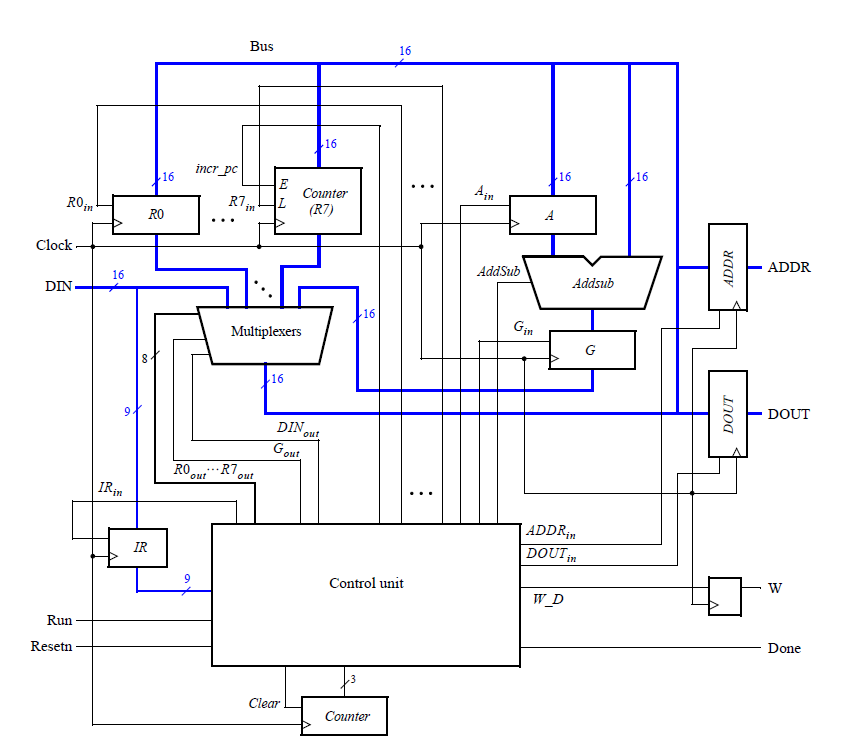
\includegraphics[width=15.3cm]{./processador_proposto}
		\caption{Processador Simplificado}
		\label{fig: processador implementado}
	\end{figure}
	
	\section{Material}
	
	\par Para realização desta prática, foi utilizado os seguintes equipamentos e softwares:
	
	\begin{itemize}
		\item ModelSim 10.1d;
		\item Quartus 13.0sp1;
		\item FPGA EP2C35F672C6 e
		\item Kernel Linux / SO Deepin 15.11.
	\end{itemize}
	
    \section{Desenvolvimento}
    
	\par O primeiro passo para o desenvolvimento do projeto, foi a identificação dos módulos a serem utilizados, que são:

	\vspace{\baselineskip}

	\begin{itemize}
		\item Registradores (13);
		\item Multiplexador;
		\item Unidade de Controle e
		\item Unidade de Lógica Aritmética - \textit{ULA}.
	\end{itemize}
	
	\vspace{\baselineskip}
	
	\par Após a implementação destes módulos e execução dos roteiros de testes individuais, foi realizado as interconexões entre os componentes como apresentado na figura \ref{fig: processador implementado}, porém devido a inclusão da instrução \textit{Move Not Zero (MVNZ)}, se fez necessário uma realimentação do registrador \textit{G} na \textit{ULA}, modificando o design final.
	
	\begin{figure}[t]
		\centering
		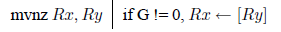
\includegraphics[width=9cm]{./mvnz}
		\caption{Instrução \textit{Move Not Zero} - \textit{MVNZ}}
		\label{fig: Move Not Zero}
	\end{figure}
    
	\section{Simulação}
	
	\par Como discutido em sala, a simulação poderia ser simplificada devido a correta execução do código na placa da Altera, sendo assim, foi simulado o funcionamento da ULA, do registrador e do multiplexador.
	
	\subsection{Unidade de Lógica Aritmética}
	
	\par Este módulo é responsável por realizar em alto nível, operações matemática como:
	
	\begin{itemize}
		\item soma ($+$);
		\item subtração ($-$);
		\item \textit{and} bit a bit (\&);
		\item deslocamento a direita ($>>$) e
		\item deslocamento a esquerda ($<<$).
	\end{itemize}
	
	\begin{figure}[H]
		\centering
		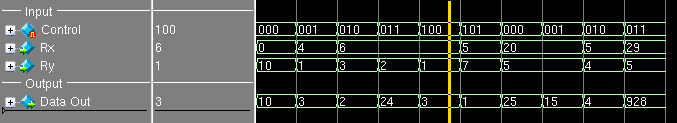
\includegraphics[width=15.3cm]{./ALU}
		\caption{Unidade de Lógica Aritmética - \textit{ULA}}
		\label{fig: ULA}
	\end{figure}

	\par Na simulação acima, foi realizado as seguintes operações:
	
	\begin{itemize}
		\item $0 + 10 = 10$
		\item $4 - 1 = 3$
		\item $6\;\&\; 3 = 2$
		\item $6 << 2 = 24$
		\item $6 >> 1 = 3$
		\item $5 < 7 = 1$, etc..
	\end{itemize}

	\subsection{Multiplexador}

	\begin{figure}[H]
		\centering
		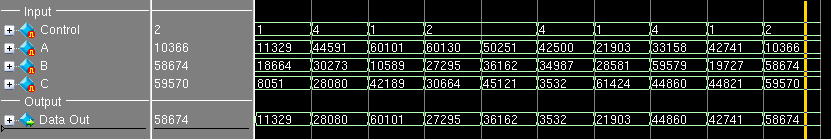
\includegraphics[width=15.3cm]{./MUX}
		\caption{Multiplexador}
		\label{fig: MUX}
	\end{figure}

	\par Como pode ser visto na figura \ref{fig: MUX}, o correto funcionamento do multiplexador consiste em escolher a saída baseado no valor da entrada de controle.

	\subsection{Registrador}
	
	\par O dado armazenado em um Registrador, só é sobrescrito quando a escrita é habilitada e tem a ocorrência da borda de subida do \textit{clock}. Seu correto funcionamento pode ser visto na figura abaixo.

	\begin{figure}[H]
		\centering
		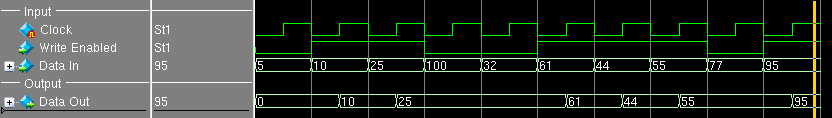
\includegraphics[width=15.3cm]{./register}
		\caption{Registrador}
		\label{fig: register}
	\end{figure}

	\section{Conclusão}
	
	\par Com a execução desta prática, foi possível reforçar os conhecimentos do funcionamento de um processador e melhorar o entendimento do paralelismo da linguagem Verilog.

\end{document}
	